The past couple of decades have seen an explosion in Internet-scale video streaming, conferencing, and analytics.
%
Over the next couple of decades, these applications will shift towards \textit{volumetric} videos.
%
In contrast to a regular video, each frame in a volumetric video represents visual information in 3D.
%
Using an augmented/mixed reality headset, a viewer can view each frame of a volumetric video in any direction from any point within the recorded environment, thus offering the viewer 6 degrees of freedom (6DoF).
%
Volumetric videos are typically captured using an array of cameras capable of recording both the color and depth of every point in the scene~\cite{holoportation}.

\begin{figure}[t]
\centering
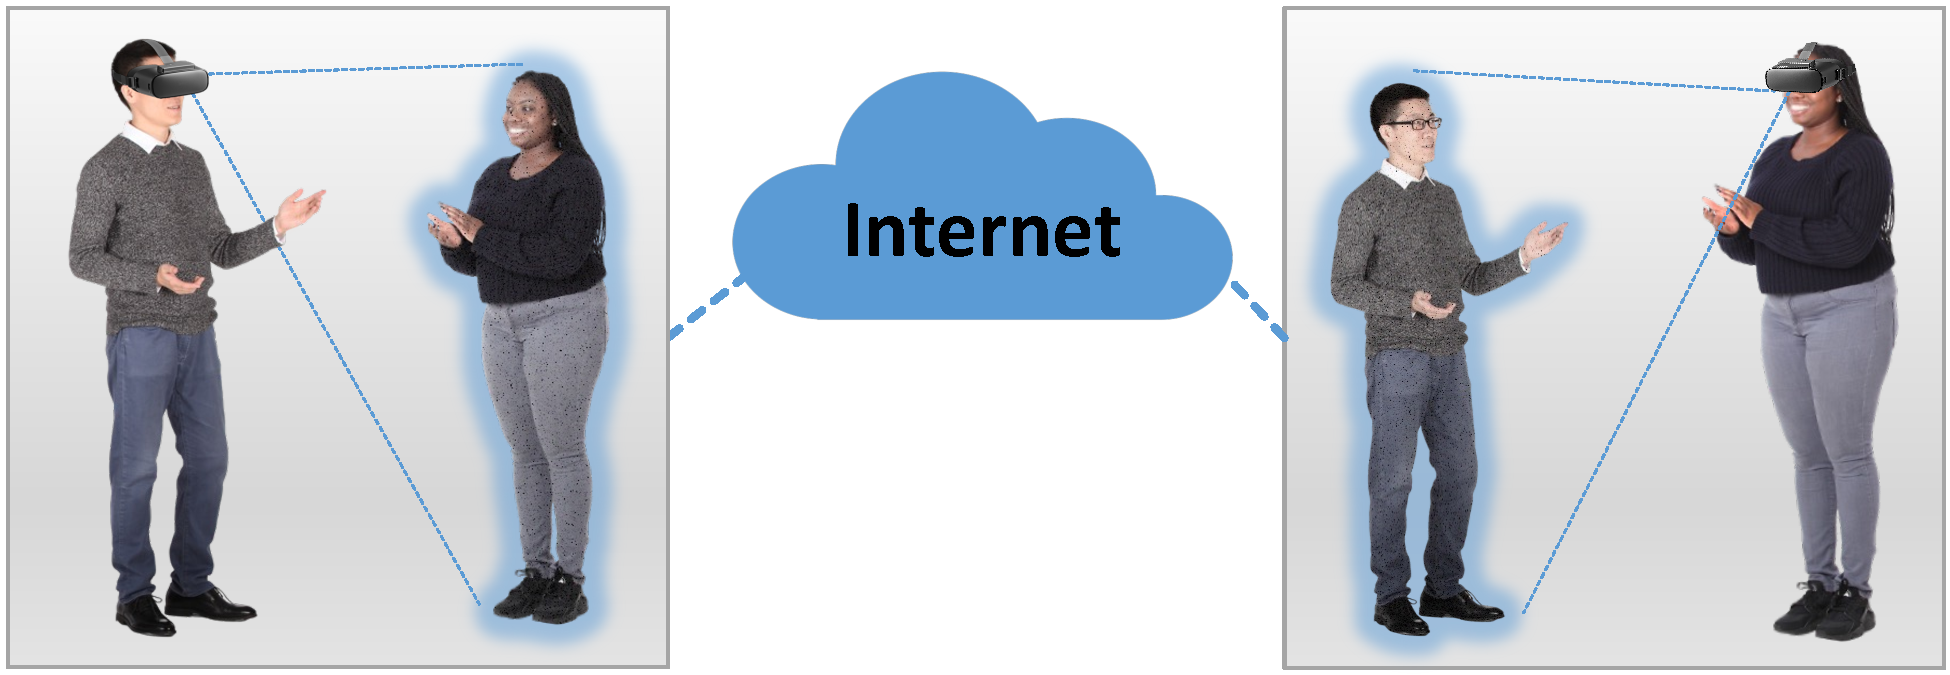
\includegraphics[width=0.8\columnwidth]{figures/AR-Depiction-0620.pdf}
\caption{A telepresence session between 2 participants using volumetric video.}
\label{fig:telepresence}
\end{figure}

%
%But, it is also feasible to learn a scene's 3D representation with cameras that can only capture color information~\cite{sfm,mildenhall22:_nerf}.

This new capability opens up a whole new class of previously infeasible applications.
%
Live volumetric streaming can offer a much more immersive experience of lectures~\cite{volumetric:education}, theater performances~\cite{volumetric:filmmaking}, telesurgery~\cite{volumetric:telemedicine}, museological storytelling~\cite{volumetric-museology}, and sports broadcasting with analytics~\cite{volumetric-golf,volumetric-sports}.
%
A major application in this domain is volumetric telepresence, where multiple participants can interact with each other in a shared virtual space or real captured space in 6 degrees of freedom (6-DoF).
%
Participants can have the illusion that they are all in the same room instead of simply seeing 2D renderings of each other (\cref{fig:telepresence}).
%
A significant extension of today's video conferencing platforms like Zoom, Microsoft Teams, and Google Meet is to extend them to provide fully immersive experiences to the participants. 

\subsection{Challenges}
Despite its promising applications, volumetric video streaming faces significant challenges:

\parab{Bandwidth Constraints.} 
%
Transmitting high-quality 3D data in the form of point cloud, mesh, or other representations requires substantial bandwidth. 
%
Volumetric video frames inherently contain detailed geometric and color information, resulting in significantly larger data sizes compared to traditional video formats. 
%
Effective compression and bandwidth management techniques are essential to handle these large data volumes within existing network constraints. 
%
The problem turns worse when streaming full-scene volumetric video compared to a portrait or single person. 
%
Moreover, current volumetric video streaming systems~\cite{vivo, groot,holoportation,livescan3d} are not bandwidth-adaptive, \ie they do not adapt to the available bandwidth of the network at a given time. 

\parab{Latency Constraints.}
%
Achieving low latency of 200-300~ms~\cite{videoconf-benchmark, conf-abr1,conf-abr2} (as achieved by today's 2D video conferencing) is particularly challenging in 3D video conferencing where delays can severely impact user's immersive experience.
%
Maintaining real-time interactions demands efficient optimization of encoding, transmission, and decoding processes. 
%
3D compression methods such as G-PCC~\cite{gpcc}, V-PCC~\cite{vpcc}, and Draco~\cite{draco} are still in their infancy and are yet to be optimized for low-latency encoding and decoding of 3D data.
%
Additionally, larger data sizes for 3D due to the low compression ratio achieved by 3D codecs increase transmission latency.

\parab{Visual Quality and Realism.} 
%
Ensuring high visual quality and realism is difficult due to potential visual artifacts introduced by current volumetric streaming approaches that primarily use point clouds as their 3D representation. 
%
Point clouds have holes and floating artifacts that can reduce realism and overall user immersion, impacting the satisfaction and effectiveness of immersive experiences. 
%
Few solutions have been proposed to use meshes instead of point clouds, but they are not yet optimized for live streaming or conferencing. 
%
Moreover, the current systems do not use recently introduced advanced rendering techniques such as Neural Radiance Fields (NeRF)~\cite{nerf} or Gaussian Splatting~\cite{gsplat} that can achieve photorealism.
%
NeRFs and Gaussian Splatting produce realistic novel view generation at the expense of high computational and memory requirements, which make them infeasible to use out of the box.

\subsection{Contributions}
%
This thesis contributes to addressing these challenges through three distinct yet complementary chapters:

\textbf{Chapter 2: \livo - Toward Bandwidth-adaptive Fully-Immersive Volumetric Video Conferencing.}
%
Chapter 2 introduces \livo, a novel conferencing system designed to efficiently stream high-quality, full-scene volumetric videos between 2 parties over the Internet.
%
\livo addresses bandwidth constraints by leveraging advanced 2D video compression techniques, rate-adaptive video codecs, and dynamic bandwidth splitting strategies.
%
It uniquely integrates view prediction and view-culling techniques to minimize transmitted data by adapting to users' real-time viewing frustum, significantly reducing bandwidth requirements without sacrificing quality. 
%
\livo carefully balances the latency for each component to match the line rate of 30 frames per second (fps) and achieves an end-to-end latency of around 250~ms.